\documentclass{beamer}
\usepackage{hyperref}
\usepackage[T1]{fontenc}
\usepackage{graphicx}
\usepackage{subcaption}


% other packages
\usepackage{latexsym,amsmath,xcolor,multicol,booktabs,calligra}
\usepackage{graphicx,pstricks,listings,stackengine}

% dummy text; remove it when working on this template
\usepackage{lipsum}
\definecolor{mycolor}{rgb}{0.1, 0.2, 0.3} % Custom RGB color

\author{\textbf{iGem IISc-Software} \\ \textbf{Ayush Raina, Rahul Chavan, Trishna}}
\title{\textcolor{yellow}{I}ntegrated \textcolor{yellow}{M}odelling of \textcolor{yellow}{PRO}TEIN Complexes \textcolor{yellow}{VI}A \textcolor{yellow}{S}ingle Shot Registration using \textcolor{yellow}{D}REAM}
\subtitle{(\textcolor{yellow}{IMPROVISeD})}



% Include 2 images in a row here in title page
\titlegraphic{
\includegraphics[width=0.5\textwidth]{images/kotak.png} \hspace{1cm} 
\includegraphics[width=0.25\textwidth]{images/igem.png}}
    
\date{\textcolor{mycolor}{\textbf{All India iGem Meet 2024 \\ July 27}}}
\usepackage{Ritsumeikan} 


% defs
\def\cmd#1{\texttt{\color{red}\footnotesize $\backslash$#1}}
\def\env#1{\texttt{\color{blue}\footnotesize #1}}
\definecolor{deepblue}{rgb}{0,0,0.5}
\definecolor{deepred}{RGB}{153,0,0}
\definecolor{deepgreen}{rgb}{0,0.5,0}
\definecolor{halfgray}{gray}{0.55}

\lstset{
    basicstyle=\ttfamily\small,
    keywordstyle=\bfseries\color{deepblue},
    emphstyle=\ttfamily\color{deepred},    % Custom highlighting style
    stringstyle=\color{deepgreen},
    numbers=left,
    numberstyle=\small\color{halfgray},
    rulesepcolor=\color{red!20!green!20!blue!20},
    frame=shadowbox,
}

\begin{document}

\begin{frame}
    \titlepage
\end{frame}

\section*{Introduction}

\begin{frame}
    \begin{enumerate}
        \item Introduction: by Rahul Chavan
    \end{enumerate}
    
\end{frame}

\begin{frame}{Integrated Modelling of Protein Complexes}
    \begin{figure}
        \centering
        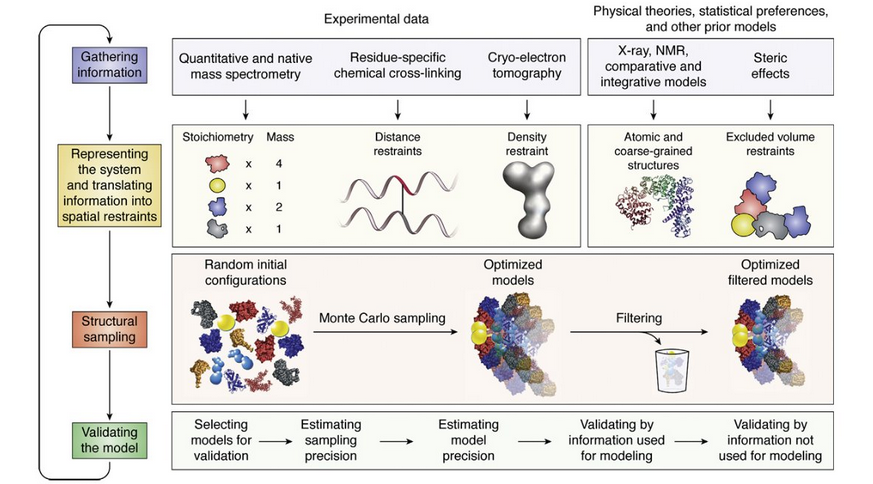
\includegraphics[width=1\textwidth]{images/imp.png}
        \caption{Flowchart representing the IMP}
        \label{fig:my_label}
    \end{figure}
\end{frame}

\begin{frame}
    \begin{figure}[h]
        \centering
        \begin{subfigure}[b]{0.3\textwidth}
            \centering
            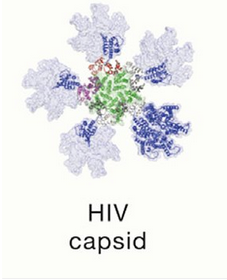
\includegraphics[width=\textwidth]{images/one.png}
            \caption{Deshmukh et al., 2013}
            \label{fig:image1}
        \end{subfigure}
        \hfill
        \begin{subfigure}[b]{0.3\textwidth}
            \centering
            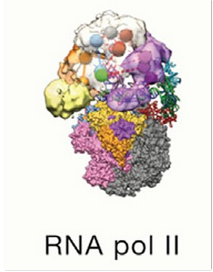
\includegraphics[width=\textwidth]{images/two.png}
            \caption{Murakami et al., 2013}
            \label{fig:image2}
        \end{subfigure}
        \hfill
        \begin{subfigure}[b]{0.3\textwidth}
            \centering
            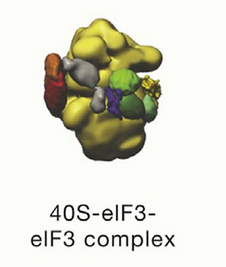
\includegraphics[width=\textwidth]{images/three.png}
            \caption{Erzberger et al., 2014}
            \label{fig:image3}
        \end{subfigure}
        
        \label{fig:three_images}
    \end{figure}
\end{frame}

\begin{frame}{Why Integrated Modelling}
    \begin{enumerate}
        \item Using new information
        \item Maximizing accuracy, precision and completeness
        \item Planning experiments
    \end{enumerate}
\end{frame}

\begin{frame}{Present Landscape}
    \begin{figure}[h]
        \centering
        \begin{subfigure}[b]{0.3\textwidth}
            \centering
            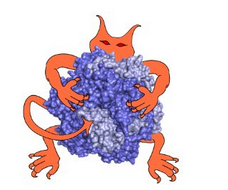
\includegraphics[width=\textwidth]{images/monster.png}
            \caption{IMP,the integrative modelling platform}
            \label{fig:image1}
        \end{subfigure}
        \hfill
        \begin{subfigure}[b]{0.3\textwidth}
            \centering
            
\includegraphics[width=\textwidth]{images/rosseta.png}
            \caption{rosetta}
            \label{fig:image2}
        \end{subfigure}
    \end{figure}

    \begin{figure}
        \centering
        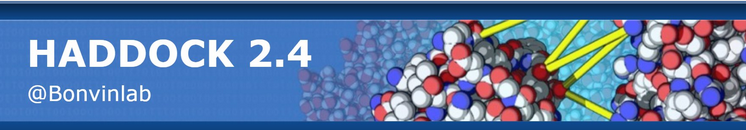
\includegraphics[width=0.8\textwidth]{images/haddock.png}
        \caption{haddock}
        \label{fig:my_label}
    \end{figure}
\end{frame}

\begin{frame}

    \begin{figure}
        \centering
        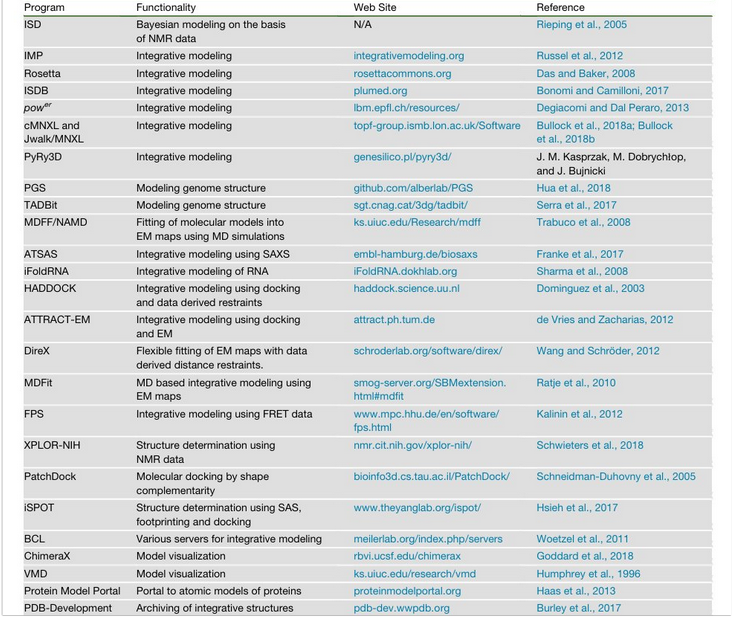
\includegraphics[width=0.8\textwidth]{images/table.png}
        \label{fig:my_label}
    \end{figure}
    
\end{frame}

\begin{frame}{Our Improvement}
    \begin{figure}
        \centering
        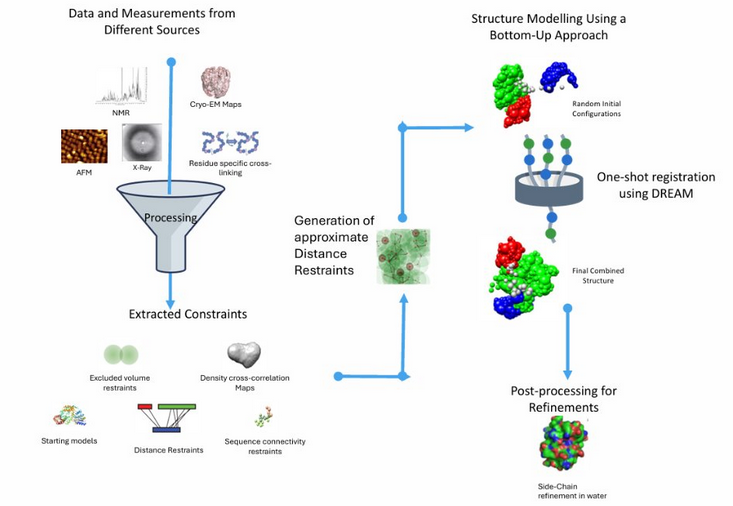
\includegraphics[width=0.7\textwidth]{images/dream.png}
        \caption{Flow Chart}
        \label{fig:my_label}
    \end{figure}

    \begin{enumerate}
        \item Single Shot Registration
        \item Scalability
    \end{enumerate}
\end{frame}

\section*{Methodology}

\begin{frame}
    \begin{enumerate}
        \setcounter{enumi}{1}
        \item Methodology
    \end{enumerate}
\end{frame}

\begin{frame}{Methodology}
    \begin{block}{Distance Restraints and Energy Assisted Modelling}
        DREAM algorithm uses distance restraints obtained from NMR data to model the structure of proteins in 3 steps:
        \begin{enumerate}
            \item \textbf{Construction of Substructures:} We divide the available distance restraints data into dense fragments and model their structure first.
        \end{enumerate}
        \pause
        \begin{figure}[h]
            \centering
            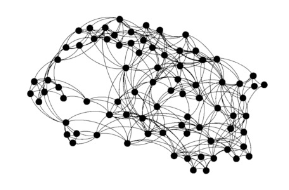
\includegraphics[width=0.35\textwidth]{images/single.png}
            \pause
            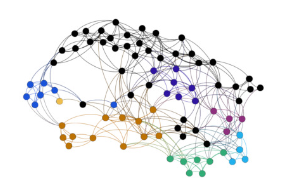
\includegraphics[width=0.35\textwidth]{images/separate.png}
            \caption{Dividing into dense fragments}
            \label{fig:my_label}
        \end{figure}
    \end{block}
\end{frame}

\begin{frame}{DREAM}
    \begin{enumerate}
        \setcounter{enumi}{1}
        \item \textbf{One Shot Registration:} We then join all the substructures into a single structure at once instead of sequential registration.
    \end{enumerate}

    \pause 

    \begin{figure}[h]
        \centering
        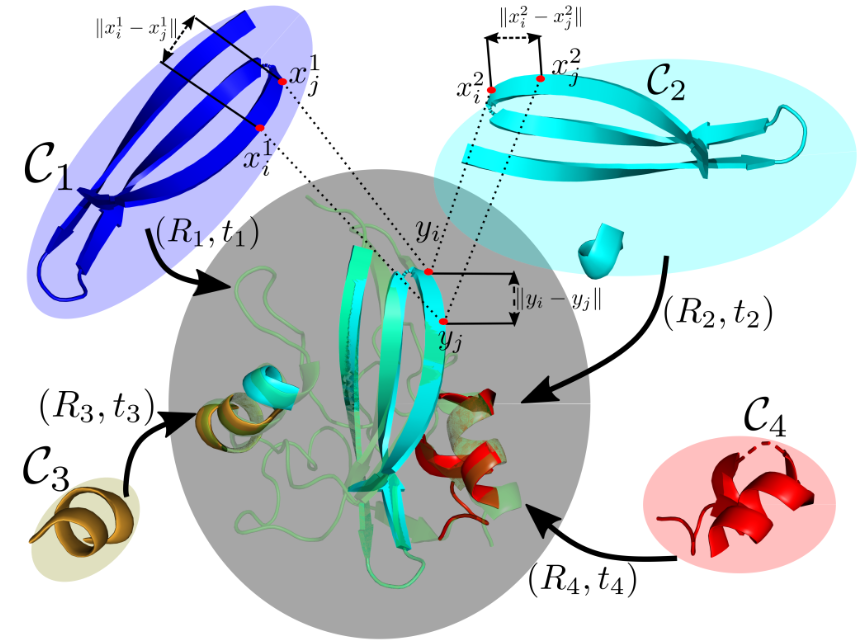
\includegraphics[width=0.45\textwidth]{images/register.png}
        \caption{One Shot Registration}
        \label{fig:my_label}
    \end{figure}

    Here $(R,t)$ denotes the rotation and translation of the substructure.
\end{frame}

\begin{frame}{DREAM}
    \begin{enumerate}
        \setcounter{enumi}{2}
        \item \textbf{Gap Filling:} Here many hybrid approaches are used to model the missing regions in the structure. This includes energy minimization, water refinement etc. 
    \end{enumerate}

    \begin{figure}[h]
        \centering
        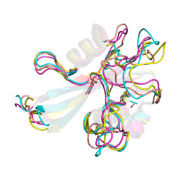
\includegraphics[width=0.4\textwidth]{images/gap1.png}
        \pause
        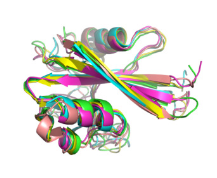
\includegraphics[width=0.4\textwidth]{images/gap2.png}
        \caption{Gap Filling}
        \label{fig:my_label}
    \end{figure}
\end{frame}

\begin{frame}{But why DREAM ?}
    \begin{itemize}
        \item Uses divide and conquer approach which increases robustness and scalability.
        \pause
        \item Reduces numerical instabilities because of the use of dense fragments.
        \pause
        \item In sequential registration, the error keeps on accumulating which is not the case in one shot registration.
    \end{itemize}
\end{frame}

\begin{frame}{Sequential vs One Shot Registration}
    \begin{figure}[h]
        \centering
        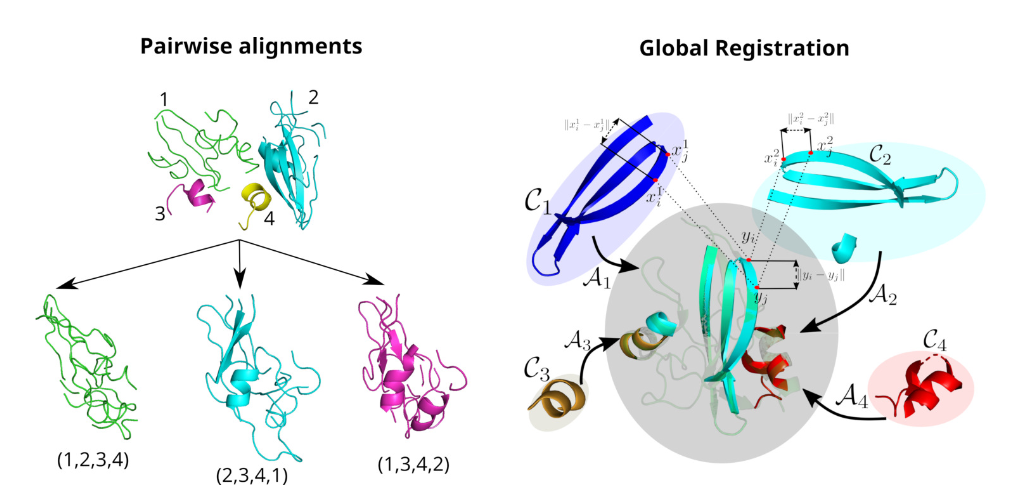
\includegraphics[width=1\textwidth]{images/seq.png}
        \caption{Sequential vs One shot registration}
        \label{fig:my_label}
    \end{figure}
\end{frame}
\begin{frame}{Integrative Modelling Platform}
    Now we already know what is IMP. It is computationally expensive and time consuming due Markov Chain Monte Carlo (MCMC) sampling. \\
    \bigskip
    \pause
    We wish to replace the computationally expensive sampling techniques to paradigms used in DREAM: \\
    \begin{itemize}
        \item Orientate the structures of subunits based on experimental evidence which is similar to substruture computation in DREAM
        \item Register the subunits in one shot while respecting the experimental evidence. (an enhancement of DREAM's registration)
    \end{itemize}
\end{frame}

\begin{frame}{How will this happen ?}
    \begin{itemize}
        \item Our substructures in this case are different kinds of proteins. \\
        \item We have cross-links data available these proteins. \\
    \end{itemize}

    Given this information, we need to do one shot registration of these proteins to model the structure of complex.

\end{frame}

\begin{frame}{}
    \begin{figure}
        \centering
        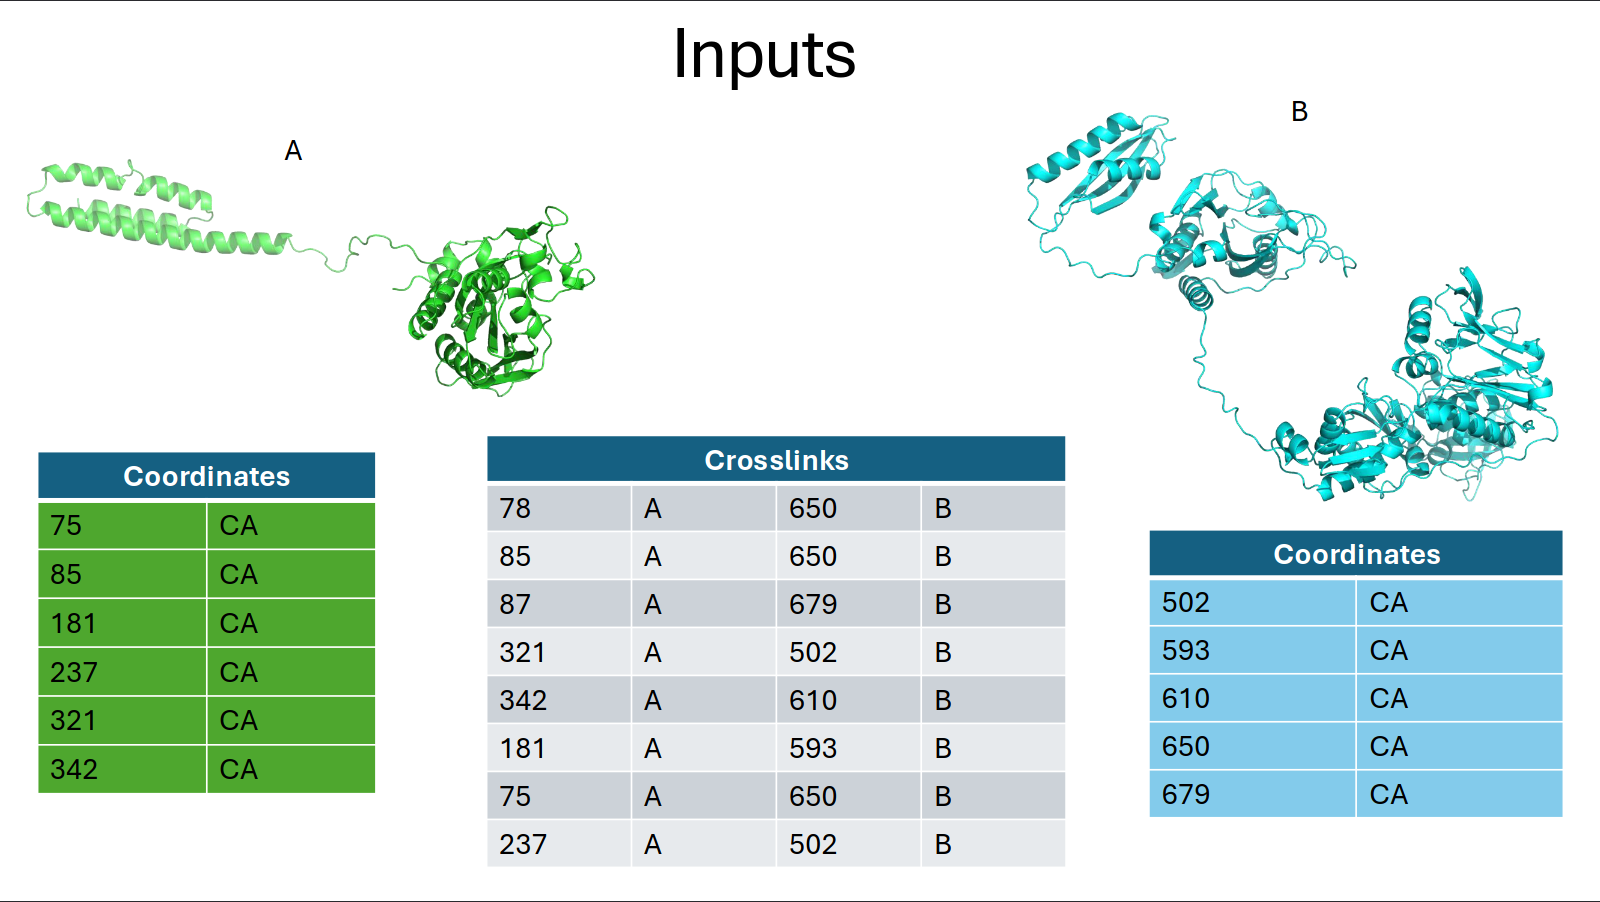
\includegraphics[width=1\textwidth]{images/local.png}
        \caption{Example of 2 proteins with cross-links data}
        \label{fig:my_label}
    \end{figure}
\end{frame}

\begin{frame}{Problem}
    \begin{figure}
        \centering
        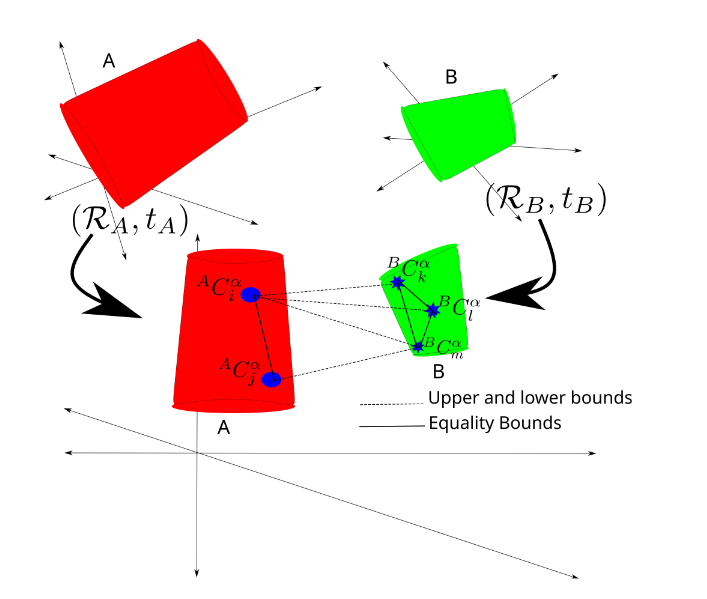
\includegraphics[width=0.7\textwidth]{images/toy1.png}
        \caption{Consider A,B as proteins and the lines as cross-links}
        \label{fig:my_label}
    \end{figure}
\end{frame}

\begin{frame}{Solution}
    \begin{figure}
        \centering
        
\includegraphics[width=0.3\textwidth]{images/A.png}
        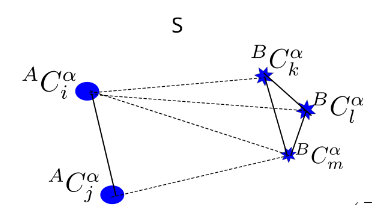
\includegraphics[width=0.3\textwidth]{images/S.png}
        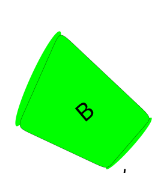
\includegraphics[width=0.3\textwidth]{images/B.png}
        \label{fig:my_label}
    \end{figure}
    Consider S as hypothetical framework. 
    \pause
    Then we can do one shot registration of A,S and B
\end{frame}

\begin{frame}{Solution}
    \begin{figure}
        \centering
        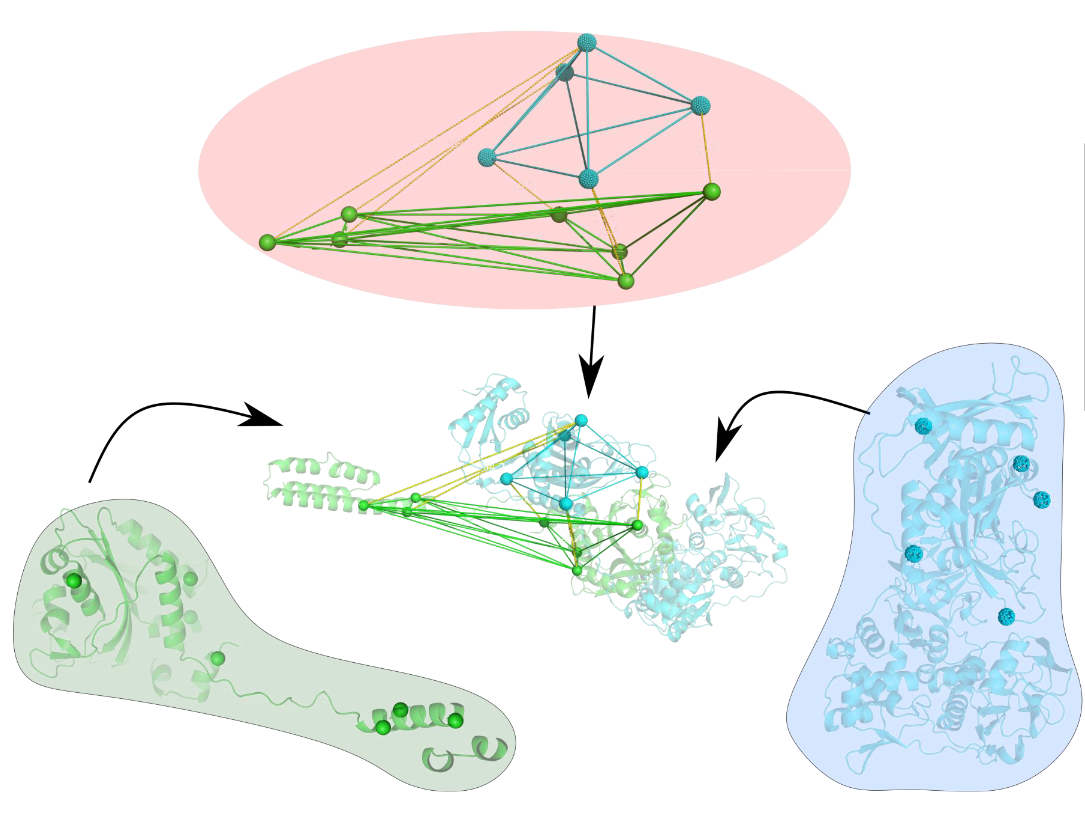
\includegraphics[width=0.7\textwidth]{images/final.png}
        \caption{One shot registration}
        \label{fig:my_label}
    \end{figure}
\end{frame}

\begin{frame}{Some Observations}
    1. In the hypothetical framework, we have all pairs of distances between C-alpha atoms in each protein. \\
    \pause
    2. For registering n proteins, only 1 hypothetical fragment is needed. So registration of $n+1$ proteins is done. \\
\end{frame}
\section*{Human Practices}

\begin{frame}
    \begin{enumerate}
        \setcounter{enumi}{2}
        \item Human Practices
    \end{enumerate}
\end{frame}

\begin{frame}{Human Practices}
    \begin{block}{The 3R's}
        \begin{itemize}
            \item Reflection
            \item Responsibility
            \item Responsiveness
        \end{itemize}
    \end{block}

    \begin{block}{Interaction with stakeholders}
        \begin{itemize}
            \item Professors
            \item Industries and Business Professionals
            \item Research Students
    
        \end{itemize}
    \end{block}
\end{frame}

\begin{frame}{Education}
    \begin{enumerate}
        \item Online and Live talks with school students about Computational Biology and AI
        \item Inclusivity of college women students, village school students across India
        \item Working with Foundations like Steam Vision Foundation and Ladakh Science Foundation
        \item Computational Biology Ideathon among colleges
        \item Structural Biology workshops for iGEMers
        \item Talks by professors from Academia
    \end{enumerate}    
\end{frame}


\begin{frame}{Our Mentors}
    \begin{figure}[h]
        \begin{subfigure}[b]{0.3\textwidth}
            \centering
            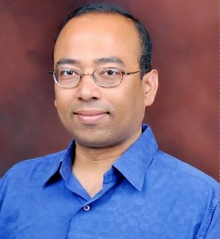
\includegraphics[width=\textwidth]{images/debnath.png}
            \caption{Prof Debnath Pal (Dept for Computational and Data Sciences)}
            \label{fig:image2}
        \end{subfigure}
        \hfill
        \centering
        \begin{subfigure}[b]{0.3\textwidth}
            \centering
            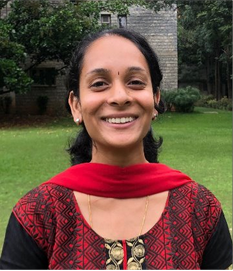
\includegraphics[width=\textwidth]{images/shruthi.png}
            \caption{Dr. Shruthi(NCBS)}
            \label{fig:image1}
        \end{subfigure}
        \hfill
        \begin{subfigure}[b]{0.3\textwidth}
            \centering
            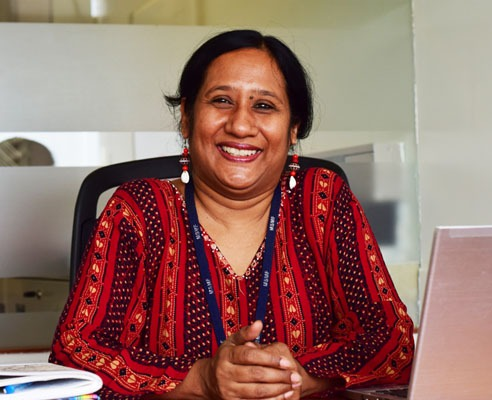
\includegraphics[width=\textwidth]{images/manjulamam.png}
            \caption{Dr. Manjula Das (MSMF)}
            \label{fig:image3}
        \end{subfigure}
    \end{figure}
\end{frame}
\section*{Summary}

\begin{frame}{To Summarize}
    Content to be added
\end{frame}

% thank you slide
\begin{frame}{Thank You!}
    \begin{center}
        \Huge Thank You!
    \end{center}
    Here are some references:
    \begin{enumerate}
        \item DREAMweb, \url{https://analyticalsciencejournals.onlinelibrary.wiley.com/doi/10.1002/pmic.202300379?af=R}
        \item Improved NMR-data-compliant protein structure modeling captures context-dependent variations and expands the scope of functional inference, \url{https://onlinelibrary.wiley.com/doi/full/10.1002/prot.26439?_gl=1*1f1toyi*_gcl_au*MjcyNjE4Nzc0LjE3MTg5MDgxOTg.}
    \end{enumerate}
\end{frame}

\end{document}

